%!TEX root=./LIVRO.tex
\chapter{Contexto, práticas e elementos de linguagem}
\markboth{Módulo 1}{}

\section*{Habilidades do SAEB}

\begin{itemize}
  \item Reconhecer artistas que contribuíram para o desenvolvimento e a disseminação de diferentes gêneros 
  e estilos nas artes visuais, dança, música e teatro.
  \item Analisar formas, gêneros e estilos distintos de artes visuais e dança, em diferentes contextos, por 
  meio de seus elementos constitutivos.
  \item Analisar a função do tema como projeto integrador das diferentes linguagens artísticas.
\end{itemize}

\section*{Habilidades da BNCC}

\begin{itemize}
  \item EF69AR01, EF69AR03, EF69AR04.
\end{itemize}


\conteudo{Para entendermos o que significa ``contexto da obra de arte'', 
primeiramente é preciso entender o que significa o verbo ``contextualizar'': 
mostrar as circunstâncias que estão ao redor de um fato, um acontecimento 
ou uma situação; entender ou interpretar algo tendo em conta as circunstâncias 
que o rodeiam.

Tendo como base esse significado, podemos entender que, para
contextualizar, é necessário analisar, interpretar e compreender uma obra
de arte, sabendo que ela foi elaborada pelos sujeitos a partir de
determinados momentos sociais, culturais e históricos em que vivem ou
viveram. A linguagem artística utilizada pelos sujeitos revela-se uma
entre outras práticas sociais e, portanto, guarda relação com a
história, com a cultura e com a sociedade de cada grupo.

Como atividade dinâmica e socialmente produzida, a linguagem artística
está sujeita a mudanças, reformulações e variantes que dizem respeito à
identidade dos sujeitos que a produzem, assim como às condições do
ambiente, aos objetivos, às funções e à época em que está sendo
empregada.

Para ajudar na contextualização de uma obra de arte, devem-se fazer perguntas como: em que data a obra foi realizada? A que período histórico a
obra está relacionada? Que artista a realizou? O que sabemos ou podemos
saber sobre esse artista? Com que finalidade a obra foi realizada? Que
os fatos sociais, políticos, econômicos, religiosos e culturais são mais
marcantes no período em que a obra foi produzida? Que relações a obra
poderia estabelecer com esses fatos? A que movimento artístico a obra
está relacionada? Quais características desse movimento estão presentes
na obra ou quais não estão?

Já as práticas na arte são o fazer artístico. Trata-se do colocar mãos à obra e experimentar e vivenciar
a arte como uma prática social, interagindo com a linguagem artística,
não somente como expectador (analista ou apreciador), mas como criador (sujeito ativo).

Por outro lado, sem intenção de esgotar os múltiplos elementos da linguagem
artística, podemos citar:

\textbf{Artes visuais}: ponto, linha, forma,
direção, cor, tom, escala, dimensão, espaço, movimento.

\textbf{Música}: altura, intensidade, timbre, melodia, ritmo. 

\textbf{Teatro}: entonações de voz, personagens, enredo, figurinos, cenário, iluminação,
sonoplastia.

\textbf{Dança}: tempo, peso, fluência, espaço, deslocamentos,
ritmos de movimento, direções.}


\section*{Atividades}

\num{1}  Para analisar e compreender uma obra de arte, o que se faz necessário?

\reduline{É necessário saber que ela foi elaborada pelos sujeitos a partir de
determinados momentos sociais, culturais e históricos em que vivem ou
viveram.\hfill}
\linhas{3}

\num{2} Como deve ser a interação do sujeito com a linguagem artística?

\reduline{O sujeito deve experimentar e vivenciar a arte como uma prática social,
interagindo com a linguagem artística, não somente como expectador --- ou seja,
analista ou apreciador ---, mas também como criador --- ou seja, sujeito ativo.\hfill}
\linhas{3}

\num{3}  Cite três elementos da linguagem artística que compõem cada item destacado a seguir.

\begin{escolha}
\item
  Artes visuais: \reduline{ponto, linha, forma, direção, cor, tom, escala, dimensão, espaço,
movimento\hfill}

\item
  Dança: \reduline{tempo, peso, fluência, espaço, deslocamentos, ritmos de movimento,
direções\hfill}

\item
  Música: \reduline{altura, intensidade, timbre, melodia, ritmo\hfill}

\item
  Teatro: \reduline{entonações de voz, personagens, narrativas, figurinos, cenário,
iluminação, sonoplastia\hfill}
\end{escolha}

\num{4} Analise os itens propostos a seguir.

\begin{itemize}
  \item Na Grécia Antiga, surgiram dois gêneros: a tragédia e a comédia.
  \item Na Grécia Antiga, a arte era apresentada em espaços especiais,
construções em forma de meia-lua.
  \item Na Itália, no final da Idade Média e início do Renascimento, surge a
\textit{commedia dell'arte}, com textos improvisados.
  \item O nome da manifestação artística deriva de um verbo grego que significa algo como ``ver'' ou ``enxergar'' e significa ``lugar de onde se vê''.
\end{itemize}

Os itens relacionam-se à que manifestação artística?

\reduline{Trata-se do teatro.\hfill}
\linhas{1}

\num{5} Divida-se com seus colegas em quatro grupos e realize a atividade proposta a seguir.

\begin{escolha}
  \item Cada grupo deverá pesquisar e estudar um período específico da história do teatro: \textbf{teatro na Antiguidade} (origens e teatro grego); \textbf{teatro na Idade Média} (teatro litúrgico e teatro medieval); \textbf{Renascimento e teatro Elisabetano} (renascimento teatral na Europa e o teatro de William Shakespeare); \textbf{teatro moderno e contemporâneo} (teatro realista, teatro do absurdo e teatro contemporâneo).
  \item Cada grupo deve pesquisar sobre o período designado, levantando informações sobre as principais características, os autores, as obras e asinfluências teatrais da época.
  \item Os grupos devem preparar uma apresentação oral, na qual cada membro do grupo terá a oportunidade de compartilhar suas descobertas.
  \item Durante a apresentação de um grupo, os demais grupos devem fazer anotações sobre os aspectos mais interessantes e fazer perguntas para estimular a discussão.
\end{escolha}

Após todas as apresentações, promovam um debate em sala de aula, abordando os seguintes pontos:

\begin{itemize}
  \item Como o teatro reflete as características culturais e sociais de cada período estudado?
  \item Quais foram as principais transformações e os avanços ocorridos ao longo da história do teatro?
  \item Como o teatro se adaptou às mudanças tecnológicas e sociais ao longo dos séculos?
  \item Quais são as influências do teatro passado no teatro contemporâneo?
  \item Como o teatro contribui para a nossa compreensão da história e da sociedade?
\end{itemize}

Redija um pequeno texto redulineando a atividade proposta como um todo.

\reduline{Ao dividir a turma em grupos e atribuir a cada um um período específico da história do teatro, proporciona-se aos alunos a oportunidade de se aprofundarem em uma área específica e se tornarem especialistas temporários. Isso não só os incentiva a pesquisar e adquirir conhecimento, mas também os encoraja a compartilhar suas descobertas com os colegas. A dicussão em sala de aula, após as apresentações, é um elemento valioso para a compreensão mais ampla do teatro ao longo do tempo. As perguntas instigam os alunos a refletir criticamente sobre as influências históricas, as transformações teatrais e o impacto do teatro em diferentes sociedades. A atividade não só promove o aprendizado de conteúdo, mas também habilidades de pesquisa, apresentação oral, trabalho em equipe e pensamento crítico.\hfill}
\linhas{5}

\num{6} O corpo se expressa nas artes visuais, na dança, na música, no
teatro e é representado de muitas formas. Sobre o assunto, analise as descrições apresentadas a seguir. Depois, pesquise e registre uma manifestação artística visual que se relaciona a cada descrição proposta.

\begin{escolha}
\item Corpo feito com poucas linhas, pouca profundidade, para expressar
a religiosidade e esconder a sensualidade de corpos reais.\\
\reduline{Possibilidade de resposta: \textit{Madonna Rucellai}, de Duccio di Buoninsegna, de 1285. Disponível em: https://tinyurl.com/nhd4b9r4.\hfill}
\linhas{1}

\item Corpo representando figura de destaque na sociedade, uma forma de
cultuar os mortos, com linhas simples e níveis retilíneos.\\
\reduline{Possibilidade de resposta: máscara funerária egípcia.\hfill}\\
 \reduline{Disponível em: https://tinyurl.com/nhd4b9r4\hfill}

\item Corpo simplificado, feito com poucas linhas, que sugere a prática de
punições daquela cultura.\\
\reduline{Possibilidade de respsota: pintura rupestre da Serra da Capivara.\hfill}\\
 \reduline{Disponível em: https://tinyurl.com/yt4zvk82.\hfill}

\item Corpo humano representado dentro das proporções corretas, para
expressar os ideais da sociedade da época, de harmonia e de 
equilíbrio.\\
\reduline{Possibilidade de resposta: \textit{Discóbolo}, de Míron, do século V a.C.\hfill}\\
 \reduline{Disponível em: https://tinyurl.com/2p8zmrre.\hfill}
\end{escolha}

\num{7} Sobre os elementos constitutivos das artes visuais, marque V para
verdadeiro e F para falso.

\begin{boxlist}
\boxitem{F} Os elementos que compõem as artes visuais são quatro: ponto, cor, linha e forma. 

\boxitem{V} O ponto é um dos elementos da linguagem visual. Uma série de pontos forma uma linha; e uma massa de pontos torna-se textura, forma ou plano. 

\boxitem{V} As linhas, sequências ordenadas de pontos, podem ser retas ou curvas. 

\boxitem{F} No espaço bidimensional, as formas têm altura, largura e profundidade. 
\end{boxlist}

\pagebreak
\num{8} Associe o gênero de cada arte visual a uma característica.

\begin{multicols}{2}
\begin{enumerate}
  \item Autorretrato.
  \item Paisagem.
  \item Natureza-morta.
  \item Retrato.
\end{enumerate}
\end{multicols}

\begin{boxlist}
  \boxitem{3} Representação de qualquer objeto inanimado.
  \boxitem{2} Representação de um local, seja no campo, seja na cidade.
  \boxitem{4} Representação de alguém por um artista.
  \boxitem{1} Representação do artista por si mesmo.
\end{boxlist}

\num{9} Leia o texto.

\begin{quote}
A linguagem audiovisual é uma combinação de elementos sonoros e visuais. Esses artefatos culturais impactam os sentidos da visão e da audição do ser humano.

\fonte{Texto escrito para este material.}
\end{quote}

Cite três elementos constitutivos das linguagens das artes visuais que
se integram à linguagem audiovisual do cinema.


\reduline{Possibilidade de resposta: cor, espaço, movimento, luz, sombra, tom, som.\hfill}
\linhas{3}

\num{10} Leia o texto sobre Augusto Boal.

\begin{quote}
\textbf{Augusto Boal}

Augusto Boal, um dos grandes nomes da dramaturgia brasileira, deixou um legado duradouro mesmo após sua morte aos 78 anos de idade. Sua abordagem inovadora do teatro como uma ferramenta de luta política e social o destacou no cenário artístico. Boal é conhecido como o criador do Teatro do Oprimido, uma técnica que coloca os espectadores como protagonistas nas encenações, rompendo as barreiras entre realidade e ficção.

Além de suas contribuições teatrais, Boal também se destacou como autor de diversas obras literárias. Seu impacto transcendeu fronteiras, conquistando prêmios e honrarias tanto no Brasil quanto no mundo. Em 2009, ano de seu falecimento, ele foi nomeado Embaixador Mundial do Teatro pela UNESCO, reconhecimento merecido por seu compromisso com a arte e sua capacidade de promover mudanças sociais através do teatro.

\fonte{Fonte de pesquisa: Luciana Console. Brasil de Fato. Há 10 anos, falecia Augusto Boal, criador do Teatro do Oprimido. Disponível em:
\emph{https://www.brasildefato.com.br/2019/05/02/ha-10-anos-falecia-augusto-boal-criador-do-teatro-do-oprimido}.
Acesso em: 08 mar. 2023.}
\end{quote}

Assim como Augusto Boal, no Brasil vários artistas contribuíram para o
desenvolvimento e a disseminação de diferentes gêneros e estilos no
teatro, nas artes visuais, na dança e na música. Faça uma pesquisa sobre os artistas elencados a seguir para escrever brevemente sobre eles e suas contribuições.

\begin{escolha}
  \item Amilcar de Castro.\\
\reduline{Amilcar de Castro (1920-2002) foi um renomado escultor brasileiro que deixou um legado marcante no mundo das artes. Sua obra é caracterizada por formas geométricas minimalistas, explorando a relação entre o vazio e o sólido, e convidando o espectador a interagir com suas esculturas. Utilizando principalmente o aço, suas peças revelam uma estética elegante e precisão técnica. Amilcar de Castro é reconhecido nacional e internacionalmente, tendo exposto em galerias e museus ao redor do mundo. Sua contribuição para a arte contemporânea brasileira é amplamente admirada e inspiradora, fazendo dele um dos artistas mais importantes do país.\hfill}
\linhas{10}

\pagebreak
  \item Deborah Colker.\\
\reduline{Deborah Colker é uma renomada coreógrafa e bailarina brasileira conhecida por suas criações inovadoras na dança contemporânea. Fundadora da Deborah Colker Companhia de Dança, ela combina movimento, música e cenografia de maneira única. Sua abordagem criativa inclui diferentes estilos e técnicas de dança, resultando em performances expressivas e técnicas. Colker colabora com artistas de diversas áreas e é reconhecida nacional e internacionalmente por sua contribuição à dança contemporânea.\hfill}
\linhas{10}

\pagebreak
  \item Pixinguinha.\\
\reduline{Pixinguinha foi um renomado músico brasileiro, conhecido por sua contribuição ao choro. Compositor, arranjador, flautista e saxofonista, ele revolucionou a música brasileira ao incorporar elementos do jazz e da música erudita. Suas composições, como "Carinhoso" e "Lamentos", são consideradas clássicos do repertório brasileiro. Pixinguinha liderou conjuntos importantes, como Os Oito Batutas, e seu legado continua influenciando músicos até hoje. Sua genialidade e contribuição o tornaram uma figura icônica da música brasileira.\hfill}
\linhas{5}
\end{escolha}


\section*{Treino}

\num{1} Leia o texto.

\begin{quote}
A instalação \textit{Canções esquecidas}, do artista australiano Michael Thomas Hill, consiste em diferentes gaiolas penduradas sobre uma área grande. Sob as gaiolas, podem-se ouvir os sons dos pássaros que habitaram Sydney, na Austrália, antes da urbanização da cidade.

\fonte{Texto escrito para este material.}
\end{quote}

Com base na descrição, percebe-se que a instalação do artista australiano

\begin{escolha}
\item
  permite o diálogo entre diferentes linguagens e a interação com o
  público.
\item
  tem como principal característica ser efêmera (só existir durante o
  tempo destinado àquela exposição).
\item
  relaciona-se à arte moderna e pode ser montada em museus, galerias e
  espaços abertos.
\item
  espera que o espectador participe passivamente da obra, comportando-se apenas como
  apreciador.
\end{escolha}

\pagebreak
\num{2} Leia o texto.

\begin{quote}
\emph{O gabinete do dr. Caligari} aponta o esgotamento físico, emocional e moral dos alemães após a Primeira Guerra Mundial. O filme, de 1920, é marcado por
cenários irreais, com foco no interior, atuações e caracterizações
exageradas, imagens com ângulos profundos e sombras marcantes, usando a
iluminação e os ângulos da câmera para criar atmosferas de medo, horror,
dor.

\fonte{Texto escrito para este material.}
\end{quote}

Com base no texto, assinale a alternativa que corresponde ao movimento artístico a que esse filme se liga.

\begin{escolha}
\item
  Impressionismo.
\item
  Expressionismo.
\item
  Surrealismo.
\item
  Neorrealismo.
\end{escolha}

\num{3}  Leia o texto.

\begin{quote}
O abstracionismo, em termos gerais, engloba formas de arte que não seguem a figuração ou a imitação do mundo. Em um sentido mais específico, o termo está associado às vanguardas europeias das décadas de 1910 e 1920, que rejeitaram a representação ilusionista da natureza. Características comuns das diferentes correntes abstratas incluem a decomposição da figura, a simplificação da forma, o uso inovador da cor, a rejeição da perspectiva e das técnicas tradicionais de modelagem, assim como a recusa aos jogos convencionais de luz e sombra.

\fonte{Fonte de pesquisa: Editores da Enciclopédia Itaú Cultural. Enciclopédia Itaú Cultural. Abstracionismo. Disponível em:
\emph{https://enciclopedia.itaucultural.org.br/termo347/abstracionismo}.
Acesso em: 08 mar. 2023.}
\end{quote}

O nome de um expoente desse estilo é

\begin{escolha}
\item Leonardo da Vinci.

\item Frida Kahlo.

\item Piet Mondrian.

\item Vincent Van Gogh.
\end{escolha}


\chapter{Materialidade e notação musical}
\markboth{Módulo 2}{}

\section*{Habilidades do SAEB}

\begin{itemize}
\item Identificar diferentes formas de registro das artes por meio de
notação ou procedimentos e técnicas de áudio e audiovisual.

\item Identificar os usos de diferentes tecnologias e recursos digitais na
produção e circulação das linguagens artísticas.

\item Analisar formas, gêneros e estilos distintos de música e teatro em
diferentes contextos, por meio de seus elementos constitutivos.

\item Analisar o papel dos profissionais e a utilização dos equipamentos
culturais no sistema de produção e circulação das artes visuais, dança,
música e teatro.
\end{itemize}

\section*{Habilidades da BNCC}

\begin{itemize}
  \item EF69AR09, EF69AR10, EF69AR16, EF69AR18, EF69AR20, EF69AR21, EF69AR22, EF69AR24.
\end{itemize}

\conteudo{O conceito de \textbf{materialidade} nas artes refere-se às características 
físicas e táteis dos materiais utilizados na criação artística. Elas desempenham um papel 
fundamental na expressão e na comunicação das ideias do artista, pois podem transmitir 
significados e sensações específicas.

As materialidades podem abranger uma ampla gama de elementos, como texturas, cores, 
formas, densidade, transparência, opacidade, peso, rigidez, flexibilidade, entre outros. 
Cada material possui propriedades distintas, e sua seleção e manipulação afetam 
diretamente a aparência e o impacto da obra de arte.

Na pintura, por exemplo, a escolha das tintas, dos pincéis e das superfícies de suporte 
pode influenciar o resultado final. O uso de pinceladas largas e visíveis cria uma 
textura mais expressiva, enquanto pinceladas finas e suaves produzem um efeito mais 
detalhado. Além disso, a escolha das cores pode evocar diferentes emoções e transmitir 
mensagens simbólicas.

Na escultura, os materiais podem variar desde a argila e a pedra até o metal e o vidro. 
Cada material possui características únicas de textura, resistência e maleabilidade, o 
que impacta o processo de criação e a forma final da escultura.

A materialidade também está presente em outras formas de arte, como a fotografia, o 
\textit{design} de moda, a instalação artística e a arte têxtil. Em cada uma dessas disciplinas, 
os artistas exploram as qualidades físicas dos materiais para transmitir suas intenções e 
estabelecer uma relação sensorial com o público.

Já a \textbf{notação musical} é a representação por meio de sinais do tom e da duração dos sons,
além da marcação das suspensões e das pausas.

A notação musical é um sistema de símbolos, um sistema gráfico, que
permite a leitura de uma composição musical, podendo representar
elementos de uma composição musical como altura, duração, intensidade e
timbre.

São exemplos de notação musical:

\begin{itemize}
\item
  \textbf{Partitura}: sistema de escrita musical tradicional e padronizado
  mundialmente, com cinco linhas e quatro espaços em branco, símbolos
  para as notas musicais, pausas, entre outros elementos.
\item
  \textbf{Tablatura}: sistema de escrita musical que informa a tecla ou o lugar
  onde o dedo do intérprete deve ser posicionado para tocar a composição
  musical, utilizando para isso letras ou números.
\end{itemize}
}

\section*{Atividades}

\num{1} Diferencie notação musical convencional e notação musical não convencional.

\reduline{A notação musical convencional é o sistema de escrita utilizado amplamente na 
música ocidental e reconhecido internacionalmente. Ele utiliza símbolos e elementos 
padronizados para representar os elementos musicais, como notas, ritmo, duração, altura, 
dinâmica e articulação. Alguns dos principais componentes da notação musical convencional 
incluem pauta, claves, notas e sinais de dinâmica. A notação musical não convencional ou 
experimental é um sistema de escrita musical que se afasta das convenções estabelecidas 
da notação convencional. É utilizado principalmente em contextos de música contemporânea, 
experimental e vanguardista, em que os compositores buscam explorar novas abordagens e 
conceitos musicais, como gráficos e símbolos abstratos, texto e instruções verbais, 
notações expandidas e notação aleatória.\hfill}

\pagebreak
\num{2} Leia o texto.

\begin{quote}
\textbf{O pai do samba: o lundu}

Acredita-se que o lundu (também conhecido como landum, lundum ou londu) seja uma dança e 
canto de origem africana trazida para o Brasil por escravos angolanos. Sua origem é 
objeto de muitas controvérsias, assim como a da modinha. O lundu foi inicialmente 
confundido com o batuque africano do qual se originou, e foi rotulado como indecente e 
lascivo em documentos oficiais que proibiam sua apresentação em ruas e teatros.

A coreografia do lundu é descrita como tendo influência espanhola devido ao levantamento 
dos braços e ao estalar dos dedos, semelhante ao uso de castanholas. Um aspecto peculiar 
da dança é a umbigada, o clímax do encontro lascivo dos umbigos do homem e da mulher. A 
marcação rítmica com palmas é um traço característico e predominante na evolução da 
dança, em um canto de estrofe-refrão típico da cultura africana.

O lundu também é um gênero de música cantada, e a mais antiga menção ao lundu-canção é 
encontrada nos versos de Caldas Barbosa, que introduziu a moda do lundu cantado a viola 
na Corte portuguesa, juntamente com a modinha brasileira.

\fonte{Fonte de pesquisa: Instituto Cravo Albin. O pai do samba: o lundu. A história da 
MPB. Disponível em: \emph{https://institutocravoalbin.com.br/o-pai-do-samba-o-lundu}. 
Acesso em: 09 mar. 2023.}
\end{quote}

Com base no texto, pode-se afirmar que

\begin{boxlist}
\boxitem{\white{X}}
  o lundu é um gênero musical erudito e uma dança brasileira de
  natureza híbrida.
\boxitem{\white{X}}
  o lundu aproveitou características de danças africanas, como o estalar
  dos dedos.
\boxitem{X}
  o dançarino, suporte e ferramenta da dança lundu, executa gestos e
  movimentos que revelam significados de seu contexto
  histórico-sócio-cultural.
\boxitem{\white{X}}
  o samba é considerado o gênero que influenciou o lundu.
\end{boxlist}

Para resolver as atividades 3 e 4, leia o texto.

\begin{quote}
O Expressionismo, movimento estético do início do século XX, teve
expoentes em diversas áreas no mundo das artes: na dança, no cinema, na
literatura, na arquitetura, na escultura e na música.

Esse movimento surgiu como uma reação à representação objetiva do
Impressionismo, no contexto histórico da Primeira Guerra Mundial e da
sociedade moderna, industrializada, buscando expressar sentimentos e
emoções, utilizando a arte para refletir o lado pessimista, sombrio e
trágico da vida.

Na dança, a apresentação solo ganha destaque e mulheres passam a ocupar
o centro dos palcos. Muitas vezes, o dançarino exercia também o papel de
coreógrafo, criando e apresentando seus próprios trabalhos. A
corporeidade é marcada pela naturalidade e pela liberdade dos movimentos.

\fonte{Texto escrito para este material.}
\end{quote}

\pagebreak
\num{3} Em que contexto e momento histórico surgiu o Expressionismo?

\reduline{O Expressionismo surgiu no início do século XX, no contexto histórico da Primeira Guerra
Mundial e da sociedade moderna, industrializada, buscando expressar
sentimentos e emoções, utilizando a arte para refletir o lado
pessimista, sombrio e trágico da vida.\hfill}
\linhas{1}

\num{4} Uma das protagonistas do Expressionismo na dança foi Isadora Duncan,
coreógrafa e bailarina norte-americana. Sobre sua técnica, marque a
alternativa correta.

\begin{boxlist}
\boxitem{\white{X}} A fluência de seus movimentos era contida.

\boxitem{X} Enfatizava o movimento natural do corpo.

\boxitem{\white{X}} Seus movimentos eram uniformes, fluidos.

\boxitem{\white{X}} Sua técnica era acadêmica e metódica.
\end{boxlist}

\num{5} Leia o texto.

\begin{quote}
\textbf{Os usos da tecnologia na arte contemporânea}

\textbf{Lisa Park} é uma artista sul-coreana especializada na criação de
``dispositivos de biofeedback''. Seu trabalho envolve o uso de 
sensores capazes de captar batimentos cardíacos e ondas cerebrais, 
bem como programação para traduzir esses sinais corporais em 
manifestações tangíveis, como vibrações sonoras que geram ondas 
em recipientes com água ou respostas luminosas em painéis. Por meio 
de suas criações, a artista explora a possibilidade de automonitoramento 
de nossos estados físicos e psicológicos.

\textbf{Gisela Motta} e \textbf{Leandro Lima} são um casal de artistas brasileiros que 
colaboram em projetos de instalações que empregam tecnologia audiovisual, 
programação e sensores. Por meio dessas obras, eles capturam momentos 
que podem ser tanto pessoais quanto relacionados ao ambiente. Sua abordagem 
busca promover a interatividade com o público e estimular a reflexão sobre 
o impacto humano na transformação dos espaços.

\fonte{Texto escrito para este material.}
\end{quote}

Vários artistas têm integrado a tecnologia a suas obras de arte. Quais
são as tecnologias e os recursos digitais citados pelo texto?

\reduline{Sensores, programação e tecnologia audiovisual.\hfill}
\linhas{3}

\pagebreak
\num{6} Associe os grupos de teatro, nacionais e internacionais, aos seus modos de criação.

\begin{multicols}{2}
\begin{enumerate}
\item \textbf{Ópera de Pequim}.

\item \textbf{Commedia Dell'Arte}.

\item \textbf{Grupo Galpão}.

\item \textbf{Bando de Teatro Olodum}.
\end{enumerate}
\end{multicols}

\begin{boxlist}
\boxitem{2} O uso de máscaras era uma forte marca desse grupo teatral. Os
espetáculos desse teatro popular aconteciam em palcos improvisados em
ruas ou praças públicas. Por meio de improvisação, música, figurinos
coloridos e acrobacias, eram apresentadas cenas que ironizavam a vida e
os costumes da época.

\boxitem{4} Criado em Salvador, em 1990, esse grupo teatral coloca em prática um
projeto que inclui representar o cotidiano da população negra, sua
religiosidade, o caráter festivo e popular, a dança, os ritmos, os
instrumentos percussivos, a memória ancestral, a estética corporal, as
formas de resistência e a ênfase no registro oral da língua.

\boxitem{3} Esse grupo teatral, criado em 1982, é uma companhia brasileira,
originária do teatro popular e de rua. Desenvolvem um teatro resultante
de diversos elementos cênicos e diversas linguagens (circo, farsa, música e
melodrama).

\boxitem{1} Teatro chinês tradicional que surgiu no final do século XVIII. Durante a
atuação, os atores mesclam canto, dança, artes marciais e acrobacias. Em
2010, esse teatro passou a fazer parte do Patrimônio Cultural Imaterial
da Humanidade.
\end{boxlist}

\num{7} Observe a fotografia.

\begin{figure}[htpb!]
\centering
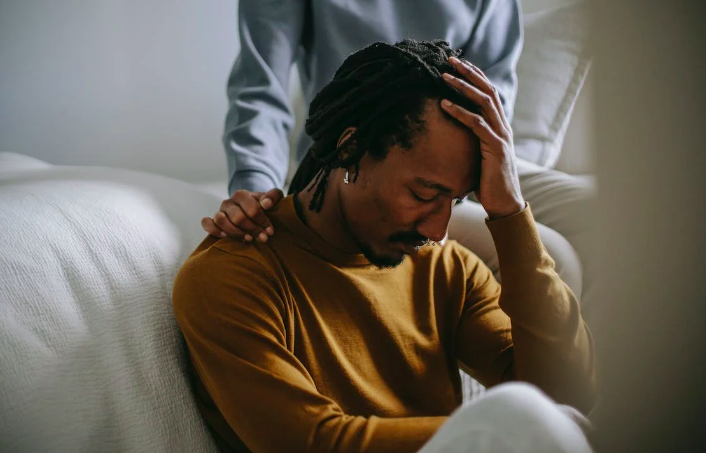
\includegraphics[width=.9\textwidth]{./media/image20.png}
\end{figure}

O que a posição do homem retratado na fotografia revela sobre seus sentimentos no momento?

\reduline{Resposta pessoal. Deverão fazer parte da resposta
sentimentos negativos, tais como angústia, ansiedade, aborrecimento,
opressão, desespero, aflição etc.\hfill}
\linhas{3}

\num{8} Leia o texto.

\begin{quote}
\textbf{O que é audiovisual?}

Pode parecer uma pergunta simples, mas você possui um conhecimento 
abrangente sobre todos os elementos envolvidos nesse tipo de linguagem? 
O audiovisual é um meio de comunicação que combina elementos visuais e 
sonoros, possibilitando a experiência simultânea de audição e visão. 
Exemplos de mídias audiovisuais incluem televisão, cinema e vídeos online. 
No entanto, para alcançar uma harmonia perfeita entre mensagem, som e 
imagem, é necessário percorrer uma série de etapas, tais como produção, 
cenografia, animação, roteirização, direção de vídeo, edição, figurino, 
iluminação, fotografia, finalização e sonorização, entre outras.

\fonte{Fonte de pesquisa: Academia Internacional de Cinema. O que é audiovisual?
Disponível em: \emph{https://www.aicinema.com.br/o-que-e-audiovisual}.
Aceso em: 09 mar. 2023.}
\end{quote}

A partir da leitura do texto, relacione o profissional às suas funções
na produção do audiovisual.

\begin{enumerate}
\item Diretor.

\item Designer de animação.

\item  Sonoplasta.

\item Roteirista.
\end{enumerate}

\begin{boxlist}
\boxitem{2} Cria sequências de imagens e efeitos especiais em 2D ou 3D.

\boxitem{3} Realiza efeitos especiais, fundos sonoros e edita áudio em sincronia com as imagens.

\boxitem{1} Aprova o roteiro, escolhe o elenco, planeja a produção.

\boxitem{4} Cria ou adapta uma narrativa para o audiovisual.
\end{boxlist}

Para resolver as atividades 9 e 10, leia o texto.

\begin{quote}
\textbf{Orquestra sinfônica}

A orquestra sinfônica contemporânea mantém a mesma formação 
estabelecida no final do século XVIII. Dependendo da composição 
a ser executada, pode ser composta por mais de 100 músicos. Ela 
é dividida em quatro grupos de instrumentos conhecidos como ``famílias'' 
ou ``naipes''.

A \textbf{família das cordas} é o grupo principal de instrumentos 
da orquestra. O violino, devido à versatilidade e ao alcance, desempenha 
um papel central nessa família. Ele é dividido em duas seções: primeiros 
violinos e segundos violinos. O \textit{spalla}, que é o primeiro violino, 
lidera o conjunto sob a orientação do maestro.

A \textbf{família das madeiras} adiciona cores ao som da orquestra. 
Surpreendentemente, a flauta, apesar de ser feita de metal, é classificada 
como um instrumento de madeira. Sua versão mais aguda, o flautim (ou 
\textit{piccolo}), produz o som mais agudo entre todos os instrumentos da 
orquestra.

A \textbf{família dos metais} é responsável pela criação de uma avalanche 
sonora na orquestra, conferindo dramaticidade e grandiosidade à obra executada. 
A trompa e o trompete adicionam agilidade sonora, enquanto o trombone e a tuba 
produzem um som majestoso.

A \textbf{família das percussões} não só fornece ritmo, mas também pontua e destaca 
trechos da peça em execução, além de trazer vibração à orquestra. Embora tenha um 
som distinto dos outros instrumentos dessa família, o piano é considerado um 
instrumento de percussão, pois o som é produzido pelas batidas dos martelos nas 
cordas.

\fonte{Fonte de pesquisa: Margaret Imbroisi e Simone Martins. História das artes. Por 
dentro da orquestra. Disponível em: \emph{https://www.historiadasartes.com/som-camera-acao/musica/os-conjuntos-musicais/}. Acesso em: 09 mar. 2023.}
\end{quote}

\num{9} Entre os parâmetros sonoros, ou seja, as propriedades do som, podemos
citar a duração, a intensidade, a altura e o timbre. Localize no texto e
trancreva um trecho que aponta um parâmetro de altura.

\reduline{Sua versão mais aguda, o flautim (ou 
\textit{piccolo}), produz o som mais agudo entre todos os instrumentos da 
orquestra.\hfill}
\linhas{6}

\num{10} A seguir, destaque as famílias de instrumentos de uma orquestra e
cite, em cada uma delas, três instrumentos que a compõem.

\reduline{\textbf{Família das cordas}: violino, viola, violoncelo, contrabaixo e harpa.
\textbf{Família das madeiras}: clarinete, requinta, clarone, flauta,~\emph{picollo}, 
cornê inglês, oboé, fagote e contrafagote. \textbf{Família dos metais}: trombone, 
trompete, trompa e tuba. \textbf{Família das percussões}: caixa clara, tímpano, pratos, 
carrilhão, xilofone, glockenspiel e piano.\hfill}
\linhas{5}

\section*{Treino}

\num{1}  Observe a fotografia.

\begin{figure}[htpb!]
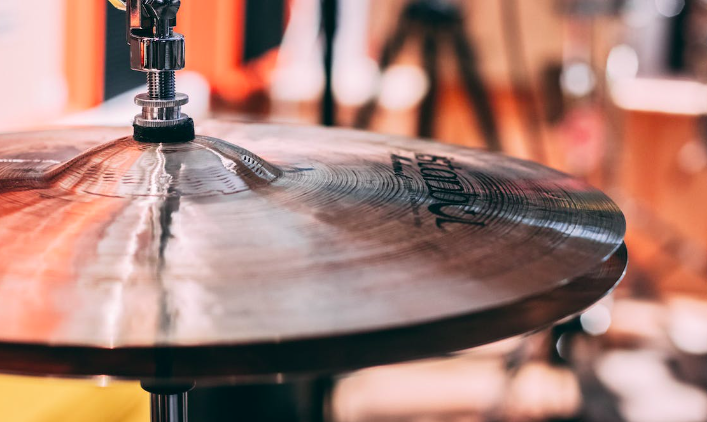
\includegraphics[width=\textwidth]{./media/image1.png}
\end{figure}

O instrumento representado faz parte do grupo dos

\begin{escolha}
\item
  aerofones, instrumentos que produzem som por meio da vibração do ar.
\item
  cordofones, instrumentos que produzem som por meio da vibração de suas
  cordas.
\item
  idiofones, instrumentos que produzem som pela própria vibração.
\item
  membranofones, instrumentos que produzem som pela vibração de uma
  membrana.
\end{escolha}

\pagebreak
\num{2} Observe a fotografia.

\begin{figure}[htpb!]
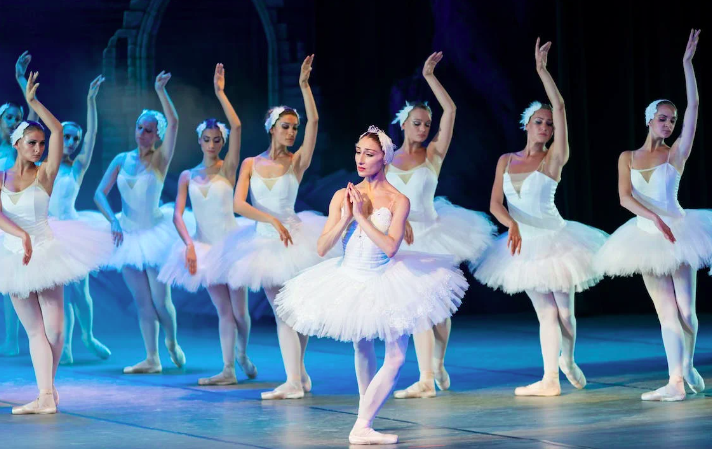
\includegraphics[width=\textwidth]{./media/image2.png}
\end{figure}

Em que período artístico surgiu a forma de arte representada na fotografia?

\begin{escolha}
\item Surgiu na Idade Média (entre os séculos V e XV).

\item Surgiu na arte renascentista (entre os séculos XIV e XVII).

\item Surgiu na Idade Contemporânea (a partir do século XVIII).

\item Surgiu na arte moderna (entre o fim do século XIX e meados do século XX).
\end{escolha}

\num{3} Leia o texto.

\begin{quote}
\textbf{Teatro do Absurdo}

O Teatro do Absurdo é uma expressão criada pelo crítico húngaro Martin Esslin (1918-2002) 
no final dos anos 1950. Essa expressão engloba peças teatrais que surgiram no período 
pós-Segunda Guerra Mundial e abordam a atmosfera de desolação, solidão e falta de comunicação 
que caracteriza o ser humano moderno. Essas peças se diferenciam radicalmente da dramaturgia 
realista tradicional, tanto em termos de estilo quanto de temas abordados. No entanto, o 
Teatro do Absurdo não é um movimento teatral organizado nem um gênero específico, mas sim uma 
classificação que destaca uma das tendências teatrais mais significativas da segunda metade 
do século XX.

\fonte{Fonte de pesquisa: TEATRO do Absurdo. In: ENCICLOPÉDIA Itaú Cultural de Arte e Cultura Brasileira. 
São Paulo: Itaú Cultural, 2023. Disponível em: \emph{http://enciclopedia.itaucultural.org.br/termo13538/teatro-do-absurdo}. Acesso em: 13 maio 2023.}
\end{quote}

\pagebreak
De acordo com o texto, o Teatro do Absurdo é

\begin{escolha}
\item
  um gênero teatral que surgiu no fim da década de 1950, no pós-Segunda
  Guerra Mundial.
\item
  um movimento teatral com traços estilísticos e temas que divergem da
  dramaturgia tradicional realista.
\item
  uma classificação que apresenta cenário realista e recriação detalhada
  de uma época ou de um lugar.
\item
  uma expressão criada para descrever a atmosfera de dor e solidão das
  peças teatrais pós-Segunda Guerra Mundial.
\end{escolha}


\chapter{Patrimônio cultural}
\markboth{Módulo 3}{}

\section*{Habilidades do SAEB}

\begin{itemize}
\item Avaliar nas linguagens artísticas a diversidade do patrimônio cultural
da humanidade (material e imaterial), em especial o brasileiro, a partir
de suas diferentes matrizes.
\item Avaliar produções que inter-relacionam diferentes linguagens
artísticas.
\item Avaliar o papel das diversas linguagens artísticas no questionamento
de estereótipos e preconceitos.
\end{itemize}

\section*{Habilidades da BNCC}

\begin{itemize}
\item EF69AR33, EF69AR34.
\end{itemize}

\conteudo{A Constituição da República Federativa do Brasil de 1988 conceitua
patrimônio cultural como sendo:

\begin{quote}
os bens de natureza material e imaterial, tomados individualmente ou em
conjunto, portadores de referência à identidade, à ação, à memória dos
diferentes grupos formadores da sociedade brasileira, nos quais se
incluem: as formas de expressão; os modos de criar, fazer e viver; as
criações científicas, artísticas e tecnológicas; as obras, objetos,
documentos, edificações e demais espaços destinados às manifestações
artístico-culturais; os conjuntos urbanos e sítios de valor histórico,
paisagístico, artístico, arqueológico, paleontológico, ecológico e
científico.

\fonte{Constituição da República Federativa do Brasil de 1988. Artigo 216. 
Disponível em: \emph{https://www.planalto.gov.br/ccivil\_03/constituicao/constituicao.htm}. 
Acesso em: 13 maio 2023.}
\end{quote}

São exemplos de bens culturais \textbf{materiais}, ou seja,
tangíveis (que se podem tocar), os que existem numa realidade material
física: cidades, sítios arqueológicos, teatros, igrejas, obras de arte,
vestimentas, documentos, fotografias, áudios e vídeos.

São exemplos de bens culturais \textbf{imateriais}, ou seja, intangíveis
(que não se podem tocar), os que não existem fisicamente ou como uma
realidade material presente o tempo todo: festas, feiras, culinária,
danças, músicas, lendas, crenças populares, rituais e idioma.

As principais matrizes brasileiras têm sua origem ou fonte,
inicialmente, nas culturas e estéticas das várias etnias indígenas
(nativos da terra), das variadas etnias de africanos escravizados e dos
europeus (primeiramente os portugueses). Depois, outras culturas e
estéticas foram fazendo parte de nossas matrizes, constituindo, assim,
uma identidade e uma cultura artística própria.

Dessa forma, para que possamos compreender e valorizar os bens culturais
materiais e imateriais do patrimônio brasileiro ou mundial se faz
necessário analisar e avaliar, não somente a própria manifestação
artística ou bem, identificando características sensoriais e artísticas
(estéticas), mas também analisar e avaliar os elementos históricos,
sociais e políticos presentes na origem e no desenvolvimento daquela
arte ao longo do tempo.}

\section*{Atividades}

\num{1} Assinale M para bem cultural material e I para bem cultural imaterial.

\begin{multicols}{2}
\begin{boxlist}
\boxitem{M} Igrejas e teatros. 

\boxitem{I} Danças e músicas. 

\boxitem{I} Crenças populares e festas. 

\boxitem{M} Áudios e vídeos. 
\end{boxlist}
\end{multicols}

\num{2}  Leia o texto.

\begin{quote}
Entendem-se por \emph{patrimônio cultural imaterial} as práticas,
representações, expressões, conhecimentos e técnicas --- junto com os
instrumentos, objetos, artefatos e lugares culturais que lhes são
associados --- que as comunidades, os grupos e, em alguns casos, os
indivíduos reconhecem como parte integrante de seu patrimônio cultural.
Esse patrimônio cultural imaterial, que se transmite de geração em
geração, é constantemente recriado pelas comunidades e pelos grupos em função
de seu ambiente, de sua interação com a natureza e de sua história,
gerando um sentimento de identidade e continuidade e contribuindo assim
para promover o respeito à diversidade cultural e à criatividade humana.

\fonte{UNESCO. Convenção para a salvaguarda do patrimônio cultural imaterial. 
Disponível em: \emph{https://unesdoc.unesco.org/ark:/48223/pf0000132540\_por}. Acesso em:
14 mar. 2023. (Adaptado.)}
\end{quote}

Escolha um campo de manifestação e cite um patrimônio cultural imaterial
de sua comunidade que deve ser salvaguardado (protegido, conservado,
preservado) e justifique sua resposta.

\textbf{Campos de manifestação}

\begin{itemize}
\item Tradições e expressões orais.

\item Expressões artísticas.

\item Práticas sociais, rituais e atos festivos.

\item Conhecimentos e práticas relacionados à natureza e ao universo.

\item Técnicas artesanais.
\end{itemize}

\pagebreak
\reduline{Resposta pessoal.\hfill}
\linhas{5}

Para resolver as atividades de 3 a 5, leia o texto.

\begin{quote}
\textbf{Literatura de Cordel agora é Patrimônio Cultural do Brasil}

{[}...{]}

A Literatura de Cordel no Brasil é o resultado de uma série de
práticas culturais em que os cantos e os contos --- e suas variantes ---
constituem as matrizes a partir das quais uma série de formas de
expressão se forjou. Na formação da cultura brasileira, da qual a
literatura de cordel faz parte, tanto indígenas quanto africanos e
portugueses adicionaram práticas de transmissão oral de suas
cosmologias, de seus contos, de suas canções. A questão da harmonia
sonora é muito ressaltada pelos poetas. Além das razões estéticas, há
uma explicação histórica para isso. No início do século XX, quando a
literatura de cordel se consolidou como um sistema editorial próprio, os
poetas desenvolveram um modo particular de comercializar seus livros nos
mercados e feiras livres. Carregavam consigo os exemplares e montavam
uma banca em que os folhetos eram exibidos. Para atrair curiosos e
compradores, os poetas costumavam cantar em voz alta trechos dos poemas,
contando dramas, tragédias, romances e sátiras. No momento mais
importante da narrativa --- quando o desfecho da história de aproximava
--- o canto era interrompido e o final da história só poderia ser
conhecido por aqueles que comprassem o folheto. Assim, a métrica
perfeita era a condição para que o poeta pudesse exercer sua performance
com maestria diante do público.

{[}...{]}

\fonte{Instituto do Patrimônio Histórico e Artístico Nacional. 
Literatura de Cordel agora é Patrimônio Cultural do Brasil. 
Disponível em: \emph{http://portal.iphan.gov.br/noticias/detalhes/4819}. 
Acesso em: 13 mar. 2023.}
\end{quote}

\num{1}  Quais são as matrizes culturais da Literatura de Cordel?

\reduline{A Literatura de Cordel recebeu contribuições das culturas africana, indígena e europeia, dos portugueses.\hfill}

\num{2}  Com base no texto que você leu, assinale V para verdadeiro e F para falso.

\begin{boxlist}
\boxitem{F} A Literatura de Cordel era vendida em mercados e feiras livres, desde sua origem.

\boxitem{F} A Literatura de Cordel é um patrimônio cultural material.

\boxitem{V} A Literatura de cordel é um patrimônio cultural imaterial.

\boxitem{F} A Literatura de Cordel é uma forma de expressão da literatura tradicional.
\end{boxlist}

\num{3} Explique, com base no texto, uma prática histórica utilizada
  pelos cordelistas para a divulgação e a comercialização da Literatura
  de Cordel.

\reduline{O aluno deve explicar o seguinte trecho: ``No início do século XX, quando a literatura de cordel se
consolidou como um sistema editorial próprio, os poetas desenvolveram um
modo particular de comercializar seus livros nos mercados e feiras
livres. Carregavam consigo os exemplares e montavam uma banca em que os
folhetos eram exibidos. Para atrair curiosos e compradores, os poetas
costumavam cantar em voz alta trechos dos poemas, contando dramas,
tragédias, romances e sátiras. No momento mais importante da narrativa
--- quando o desfecho da história de aproximava --- o canto era
interrompido e o final da história só poderia ser conhecido por aqueles
que comprassem o folheto.''\hfill}
\linhas{2}

Para resolver as atividades 6 e 7, leia o texto.

\begin{quote}
\textbf{Roda de capoeira recebe título de Patrimônio Cultural Imaterial da Humanidade}

Dança, luta, símbolo de resistência e uma das manifestações culturais mais 
conhecidas no Brasil, a roda de capoeira recebeu [em 26 de novembro de 2014] 
o título de Patrimônio Cultural Imaterial da Humanidade da Organização das 
Nações Unidas para a Educação, a Ciência e a Cultura (Unesco).

Após votação durante a 9ª Sessão do Comitê Intergovernamental para a Salvaguarda 
do Patrimônio Imaterial, em Paris, a roda de capoeira ganhou oficialmente o título.

A presidenta do Instituto do Patrimônio Histórico e Artístico Nacional (Iphan), 
Jurema Machado, presente na sessão do comitê, explicou que as políticas de patrimônio 
imaterial não existem apenas para conferir títulos, mas para que os governos 
assumam compromissos de preservação de seus bens culturais, materiais e imateriais.

``O reconhecimento representa um tributo à capoeira como manifestação cultural 
importante, que durante séculos foi criminalizada, além de dar visibilidade 
internacional. Além disso, reconhece que o Brasil tem políticas públicas para cuidar 
do seu patrimônio cultural'', disse Jurema {[}...{]}.

Segundo ela, um bem registrado como Patrimônio Cultural Imaterial da Humanidade 
garante mais respaldo ao governo para apoiar, com recursos públicos, iniciativas 
de preservação do bem cultural, com o incentivo à transmissão do conhecimento e a 
formas de organização dos capoeiristas. A roda de capoeira é reconhecida como 
patrimônio cultural pelo Iphan desde 2008.

{[}...{]}

\fonte{Ana Cristina Campos. Agência Brasil. Roda de capoeira recebe título de 
Patrimônio Cultural Imaterial da Humanidade. Disponível em: 
\emph{https://agenciabrasil.ebc.com.br/cultura/noticia/2014-11/roda-de-capoeira-recebe-titulo-de-patrimonio-cultural-imaterial-da}. Acesso em: 13 maio 2023.}
\end{quote}

\pagebreak
\num{6} Mesmo após a abolição da escravatura, a prática da capoeira continuou
  sendo vista como subversiva e, apenas em 1937, deixou de ser considerada
  criminosa pelo Código Penal brasileiro. Destaque no texto a informação
  que reforça essa afirmativa.

\reduline{``O reconhecimento representa um tributo à capoeira como manifestação cultural 
importante, que durante séculos foi criminalizada, além de dar visibilidade 
internacional.''\hfill}
\linhas{3}

\num{7} Em que período histórico, social e político surgiu a roda de
  capoeira?

\reduline{A roda de capoeira surgiu no século XVII, no período colonial brasileiro.\hfill}
\linhas{5}

\num{8} Relacione os patrimônios imateriais com seus respectivos livros de
  registro no Instituto do Patrimônio Histórico e Artístico Nacional
  (IPHAN), tendo como base a descrição de cada um.

\begin{enumerate}
\item Frevo.

\item Ofício das Baianas de Acarajé.

\item Complexo Cultural do Boi Bumbá do Médio Amazonas e Parintins.

\item Feira de Caruaru.
\end{enumerate}

\begin{boxlist}
\boxitem{3} \textbf{Livro de registro das celebrações.} Reúne os rituais e
festas que marcam vivência coletiva, religiosidade, entretenimento e
outras práticas da vida social, que marcam a vivência coletiva de um
grupo social, sendo considerados importantes para a sua cultura, memória
e identidade, e acontecem em lugares ou territórios específicos.

\boxitem{4} \textbf{Livro de registro dos lugares.} Recebe as inscrições dos
lugares que possuem sentido cultural diferenciado para a população
local, onde são realizadas práticas e atividades de naturezas variadas,
tanto cotidianas quanto excepcionais, tanto vernáculas (próprias do país
ou região) quanto oficiais.

\boxitem{1} \textbf{Livro de registro das formas de expressão.} Recebe 
inscrição das formas de comunicação associadas a determinado grupo
social ou região, desenvolvidas por atores sociais reconhecidos pela
comunidade e em relação às quais o costume define normas, expectativas e
padrões de qualidade. Trata-se da apreensão das performances culturais
de grupos sociais, como manifestações literárias, musicais, plásticas,
cênicas e lúdicas, que são por eles consideradas importantes para a sua
cultura, memória e identidade.

\boxitem{2} \textbf{Livro de registro dos saberes.} Reúne os 
conhecimentos tradicionais associados a atividades desenvolvidas 
por atores sociais reconhecidos como grandes
conhecedores de técnicas, ofícios e matérias-primas que identifiquem um
grupo social ou uma localidade. Geralmente estão associados à produção
de objetos ou à prestação de serviços que podem ter sentidos práticos ou
rituais.
\end{boxlist}

Para resolver as atividades 9 e 10, leia o texto.

\begin{quote}
\textbf{Patrimônio}

O patrimônio pode ser dividido em duas categorias principais: \textbf{patrimônio 
natural} e \textbf{patrimônio cultural}.

O patrimônio natural compreende as riquezas encontradas no solo e no subsolo, 
como florestas e depósitos minerais. O conceito de patrimônio cultural tem sido 
ampliado à medida que a definição de cultura é revisada. Atualmente, há um 
consenso de que o patrimônio cultural abrange muito mais do que apenas bens 
materiais; também engloba aspectos imateriais. Ele não se limita apenas às 
manifestações artísticas, mas abrange todo o conjunto de atividades humanas, 
refletindo não apenas a cultura das classes privilegiadas, mas também a cultura 
dos menos favorecidos.

O patrimônio deixou de ser definido apenas por edifícios que abrigaram reis, condes 
e marqueses, bem como pelos objetos que lhes pertenceram. Agora, ele é entendido 
como o conjunto de utensílios, hábitos, costumes, crenças e estilo de vida cotidiano 
de todos os segmentos que compuseram e compõem a sociedade ao longo do tempo.

\fonte{Texto escrito para este material.}
\end{quote}

\num{9} De acordo com o texto, o que era considerado patrimônio cultural na
  visão tradicional e eurocêntrica (com tendência a interpretar o mundo
  segundo os valores do ocidente europeu)?

\reduline{Os bens que representavam a cultura das classes mais abastadas.\hfill}
\linhas{3}

\pagebreak
\num{10} De acordo com o texto, o que é considerado patrimônio cultural na
  atualidade?

\reduline{Na atualidade, é considerado como patrimônio cultural o conjunto de
todos os utensílios, hábitos, usos e costumes, crenças e forma de vida
cotidiana de todos os segmentos que compuseram e compõem a sociedade ao
longo dos anos.\hfill}
\linhas{3}

\section*{Treino}

\num{1} Leia o texto.

\begin{quote}
{[}...{]} é um elemento estruturante de uma manifestação cultural, espaço e tempo, 
[em que] se expressam simultaneamente o canto, o toque dos instrumentos, a dança, 
os golpes, o jogo, a brincadeira, os símbolos e rituais de herança africana 
--- notadamente banto --- recriados no Brasil. {[}...{]}

\fonte{Instituto do Patrimônio Histórico e Artístico Nacional. Patrimônio imaterial.
Disponível em: \emph{http://portal.iphan.gov.br/pagina/detalhes/541}.
Acesso em: 13 maio 2025.}
\end{quote}
  
Essa descrição refere-se

\begin{escolha}
\item ao carimbó.
\item ao frevo.
\item ao samba de roda do recôncavo baiano.
\item à roda de capoeira.
\end{escolha}

\num{2} Leia o texto.

\begin{quote}
Os processos de globalização e de transformação social, ao mesmo tempo
em que criam condições propícias para um diálogo renovado entre as
comunidades, geram também, da mesma forma que o fenômeno da
intolerância, graves riscos de deterioração, desaparecimento e
destruição do patrimônio cultural imaterial, devido em particular à
falta de meios para sua salvaguarda.

\fonte{UNESCO. Convenção para a salvaguarda do patrimônio cultural imaterial. 
Disponível em: \emph{https://unesdoc.unesco.org/ark:/48223/pf0000132540\_por}. Acesso em:
14 mar. 2023.}
\end{quote}

\pagebreak
Cada alternativa a seguir contém um depoimento retirado de uma notícia divulgada
no Brasil. Assinale aquela que apresenta o fenômeno descrito no texto.

\begin{escolha}
\item
\begin{quote}
Foi lamentável a imagem da escultura do meu avô, Ariano, no chão, um 
ato de depreciação do patrimônio público e até de nossa cultura.

\fonte{Mhatteus Sampaio. G1. Disponível em: \emph{https://g1.globo.com/pe/pernambuco/noticia/2020/09/22/depreciacao-do-patrimonio-publico-e-ate-de-nossa-cultura-diz-neta-de-ariano-suassuna-sobre-escultura-depredada-no-recife.ghtml}.
Acesso em: 14 mar. 2023.}
\end{quote}

\item
\begin{quote}
Nem mesmo as obras que valorizam a nossa cultura foram poupadas. Nove 
monumentos e diversos brasões, principalmente nas pontes e no Bairro 
do Recife, também sofreram ações de depredação e furtos, somando um 
prejuízo de quase R\$ 400 mil, que só não foi maior porque algumas 
peças foram resgatadas.

\fonte{Diário de Pernambuco. Disponível em: \emph{https://www.diariodepernambuco.com.br/noticia/vidaurbana/2023/01/vandalismo-e-furtos-de-patrimonio-publico-causaram-prejuizos-de-r-2-4.html}.
Acesso em: 14 mar. 2023.}
\end{quote}

\item
\begin{quote}
Hoje estamos todos juntos comemorando, vestidos de branco, pedindo 
paz e respeito para a nossa religião. Estamos reivindicando um direito 
que já é nosso e está escrito na Constituição mas, infelizmente, não 
funciona assim.

\fonte{Maysa Polcri. Correio. Disponível em: \emph{https://www.correio24horas.com.br/noticia/nid/povo-do-axe-vai-as-ruas-pelo-fim-da-intolerancia-religiosa/}.
Acesso em: 14 mar. 2023.}
\end{quote}

\item
\begin{quote}
A gestão municipal gasta muito para recuperar espaços e apagar 
pichações praticamente todos os dias. {[}...{]} O custo e o 
dano desses atos de vandalismo infelizmente vêm para a própria 
população, pois deixamos de fazer novas obras, para recuperar 
outras.

\fonte{Correio. Disponível em: \emph{https://www.correio24horas.com.br/noticia/nid/monumento-cleriston-andrade-e-pichado-mais-uma-vez}.
Acesso em: 14 mar. 2023}
\end{quote}

\end{escolha}

\num{3} Leia o texto.

\begin{quote}
\textbf{Conjunto Moderno da Pampulha -- Belo Horizonte (MG)}

O Conjunto Moderno da Pampulha, situado em uma das regiões mais
tradicionais de Belo Horizonte (MG), recebeu o título de Patrimônio
Mundial, no dia 16 de julho de 2016. {[}...{]}

Formado por quatro edifícios articulados em torno do espelho d'água de
um lago urbano artificial, é composto pela Igreja de São Francisco de
Assis, o Cassino (atual Museu de Arte da Pampulha), a Casa do Baile
(Centro de Referência em Urbanismo, Arquitetura e Design de Belo
Horizonte) e o Iate Golfe Clube (Iate Tênis Clube), bens construídos
entre 1942 e 1943. Completam esse patrimônio cultural os painéis em
azulejos criados por Candido Portinari, esculturas de artistas renomados
como Alfredo Ceschiatti e José Alves Pedrosa, e os jardins planejados
pelo paisagista Roberto Burle Marx.

{[}...{]}

\fonte{Instituto do Patrimônio Histórico e Artístico Nacional. 
Disponível em \emph{http://portal.iphan.gov.br/pagina/detalhes/820}.
Acesso em: 14 mar. 2023.}
\end{quote}

Segundo sua natureza, como pode ser classificado o conjunto descrito no texto?

\begin{escolha}
\item
  Patrimônio arqueológico.
\item
  Patrimônio paisagístico.
\item
  Patrimônio etnográfico.
\item
  Patrimônio das artes aplicadas.
\end{escolha}






